\chapter{PJ1-Football Rob}
\section{球場建立}
\begin{figure}[hbt!]
\begin{center}
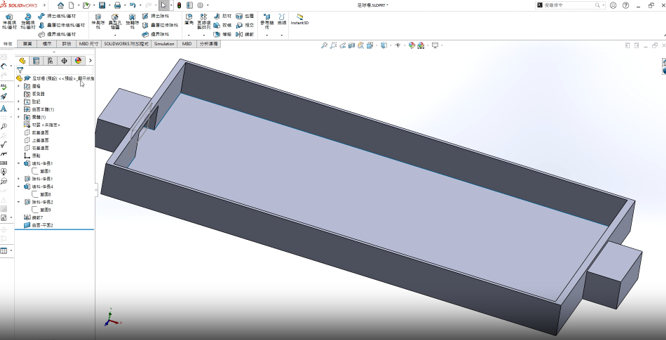
\includegraphics[width=16cm]{球場}
\caption{\Large 球場繪製}\label{球場繪製}
\end{center}
\end{figure} 
如 (圖.\ref{球場繪製}) 使用SolidWorks繪製我們足球場。
接著將繪製完成將球場STL檔匯入Coppeliasim並調整位置,但需將球場的Collidable、Measurable開啟
不過Detectable需關閉,不然球門的感測器會偵測到球場本體。如 (圖.\ref{導入球場}) 
\begin{figure}[hbt!]
\begin{center}
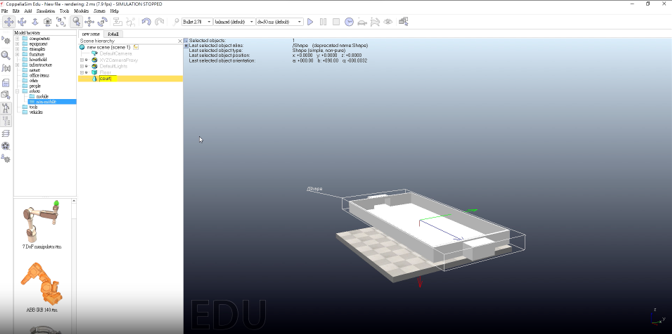
\includegraphics[width=16cm]{球場2}
\caption{\Large 導入球場}\label{導入球場}
\end{center}
\end{figure} 
\newpage

接著依序加入感測器(圖.\ref{加入感測器}) 、bubbleRob(圖.\ref{加入bubbleRob}) 、足球本體(圖.\ref{加入球體})並且定義位置。
\begin{figure}[hbt!]
\begin{center}
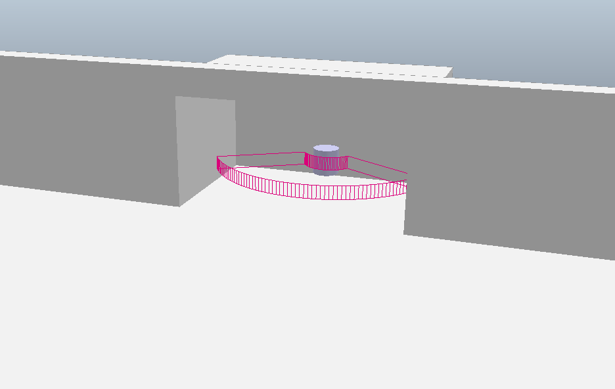
\includegraphics[width=16cm]{感測器}
\caption{\Large 加入感測器}\label{加入感測器}
\end{center}
\end{figure} 
\begin{figure}[hbt!]
\begin{center}
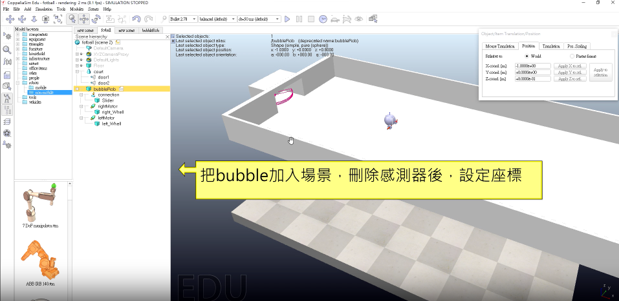
\includegraphics[width=16cm]{bubbleRob}
\caption{\Large 加入bubbleRob}\label{加入bubbleRob}
\end{center}
\end{figure} 
\begin{figure}[hbt!]
\begin{center}
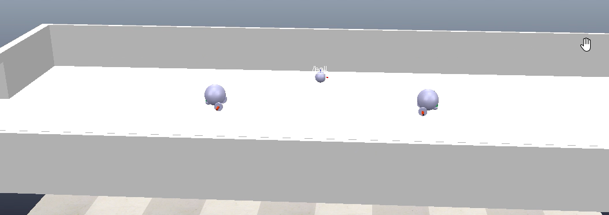
\includegraphics[width=16cm]{球體}
\caption{\Large 加入球體}\label{加入球體}
\end{center}
\end{figure} 
\newpage